\documentclass[11pt]{article}
\usepackage[margin=1.1in]{geometry}
\usepackage{amsmath,amssymb,amsthm,bm,booktabs,graphicx,enumitem,microtype,xcolor}
\usepackage[round]{natbib}
\usepackage[colorlinks=true,allcolors=blue!55!black]{hyperref}
\theoremstyle{plain}
\newtheorem{theorem}{Theorem}\newtheorem{lemma}{Lemma}\newtheorem{proposition}{Proposition}
\theoremstyle{definition}
\newtheorem{assumption}{Assumption}
\theoremstyle{remark}
\newtheorem*{intuition}{Intuition}\newtheorem*{stats}{Connection to statistics}\newtheorem*{remark}{Remark}
\newcommand{\E}{\mathbb{E}}\newcommand{\R}{\mathbb{R}}\newcommand{\N}{\mathcal{N}}
\newcommand{\corr}{\mathrm{corr}}\newcommand{\GP}{\mathcal{GP}}\newcommand{\Var}{\mathrm{Var}}
\newcommand{\Cov}{\mathrm{Cov}}\newcommand{\diag}{\mathrm{diag}}\newcommand{\tr}{\mathrm{tr}}
\title{\textbf{Structure as Covariance}\\[2pt]\large A Statistician's Walkthrough of Graph-Kernel Active Retrieval}
\author{Robert Richardson}
\date{\today}

\begin{document}
\maketitle
\begin{abstract}
\noindent This is an extended, self-contained companion to the paper ``Structure as Covariance: When a Graph Kernel
Helps Budget-Limited Active Retrieval.'' It is written for statisticians who are not steeped in the machine-learning
retrieval literature. Where the conference paper compresses, this document expands: it explains the applied setting
in plain terms, sets up the statistical model from first principles, and derives every result slowly---the Gaussian
process posterior (which is kriging), the graph kernel (which is a Gaussian Markov random field / conditional
autoregressive prior), the ``correlation-form'' normalization (a hub-variance calculation), the acquisition rule (a
Bayesian experimental-design choice), and the alignment law (a stochastic-block-model probability computation). At
each step I flag the connection to a piece of statistics you already know. Nothing here contradicts the conference
paper; it is the long version of the same story.
\end{abstract}

\tableofcontents
\bigskip

\part*{Part I. The problem, in plain terms}
\addcontentsline{toc}{section}{Part I. The problem, in plain terms}

\section{The one-paragraph version, for a statistician}
A system answers questions by first \emph{retrieving} a handful of text passages from a large corpus and then
feeding them to a language model. For hard ``multi-hop'' questions, the crucial passage is not the one that looks
like the question; it is a \emph{bridge} that supplies a linking fact, and it sits buried among look-alike
distractors. We are allowed to pay for a small number of expensive ``relevance judgments'' (each is a language-model
call) and must decide \emph{which} passages to spend them on, and how each judgment should update our beliefs about
the others. That is a sequential experimental-design problem on a latent relevance surface. Our thesis is a
decomposition: the \emph{mean} of that surface should come from cheap semantic similarity, but its \emph{covariance}
should come from a graph on the corpus. The graph is a bad way to \emph{rank} passages but an excellent way to
\emph{propagate a judgment}: judging one passage lifts our belief about its graph-neighbours, and that is exactly
how a buried bridge gets surfaced. The rest of this document makes each italicized word precise.

\section{The applied setting, explained from scratch}\label{sec:setting}
You can skip this section if the words ``retrieval-augmented generation,'' ``embedding,'' and ``LLM-as-judge'' are
already familiar. If not, here is the minimum.

\paragraph{Large language models (LLMs) and retrieval-augmented generation (RAG).} A language model is a function
that maps a text prompt to a text continuation. It has no reliable memory of specific facts, so in practice one
\emph{retrieves} relevant documents and pastes them into the prompt; the model then answers using them. This is
retrieval-augmented generation \citep{lewis2020rag}. The quality of the final answer is bottlenecked by whether the
retrieved passages actually contain the needed evidence.

\paragraph{Passages, questions, and ``gold.''} The corpus is chopped into short \emph{passages} (a paragraph each).
For a benchmark question we are told which passages are the true supporting evidence; call these the \emph{gold}
passages. Retrieval quality is scored by whether the gold passages appear near the top of the returned list
(\emph{recall@$k$}: the fraction of gold passages in the top $k$).

\paragraph{Multi-hop questions and the ``bridge.''} A \emph{multi-hop} question needs a chain of facts. ``In what
city was the director of \emph{Inception} born?'' requires (1)~a passage naming the director (Christopher Nolan) and
(2)~a passage giving \emph{his} birthplace. Passage~(2)---about Nolan's biography---may not mention \emph{Inception}
at all. It is the \emph{bridge}: necessary, but textually dissimilar to the question. This is the whole difficulty.
A first hop is easy to find; the bridge is not.

\paragraph{Embeddings and the first-stage retriever.} Each passage and the question are mapped to unit vectors
$v_i\in\R^d$ (``embeddings'') so that cosine similarity $v_i^\top v_q$ measures topical closeness. A fast
first-stage retriever returns the top $N$ passages by cosine similarity to the question. By construction the bridge
has \emph{low} cosine similarity to the question, so it is deep in this list or buried among distractors. Cosine
similarity is a fine \emph{prior} but it cannot, by itself, pull the bridge up.

\paragraph{The LLM relevance judge, and why it costs.} We can ask a language model, for a specific passage, ``is
this passage relevant to answering the question?'' This is far more accurate than cosine similarity---in particular
a suitably prompted judge can recognize a bridge---but each such judgment is a separate, slow, monetarily nontrivial
model call. So we have a \emph{judgment budget} $B$: a small number (often $B\le 10$) of passages per question that
we may submit to the judge. Everything hinges on spending those judgments well.

\paragraph{A subtlety that matters: the judge must be ``hop-aware.''} A naive judge (``does this passage answer the
question?'') is \emph{bridge-blind}: the bridge does not answer the question, so the judge grades it $0$. In our
data the naive judge recovers only $35\%$ of gold passages. A judge prompted to also credit passages that ``supply
a linking entity or intermediate fact needed to reach the answer'' recovers $84\%$. We use graded labels
$y\in\{0,\tfrac12,1\}$ (irrelevant / related / directly-supporting). This is a data-quality point, not a modelling
one, but without it there is nothing to propagate.

\begin{stats}
Strip the vocabulary and this is a familiar animal. We have a large index set (the pool of $N$ candidate passages),
a cheap noisy covariate at every location (cosine similarity), an expensive accurate measurement we can take at a
few locations (the judge), and a budget. We want to choose measurement locations sequentially to best recover a
latent field (true relevance). That is \emph{spatial sampling / active learning / Bayesian experimental design}.
The only unusual ingredient is that the ``spatial'' dependence is not geographic---it is a graph on the corpus.
\end{stats}

\section{The statistical reframing}\label{sec:reframe}
Fix a query. The first-stage retriever has handed us $N$ candidate passages, indexed $i=1,\dots,N$, each with an
embedding $v_i$ and a cosine similarity to the query. Let $f_i\in\R$ be a latent ``relevance'' for passage $i$: high
if $i$ is gold, low otherwise. We never observe $f$ directly. We observe:
\begin{itemize}[topsep=2pt,itemsep=1pt]
\item for \emph{every} $i$, a cheap prior signal (cosine similarity), which we will turn into a prior mean $m_i$;
\item for a chosen budget-limited subset $J\subseteq\{1,\dots,N\}$ with $|J|=B$, noisy graded judge labels $y_j$.
\end{itemize}
The task is to rank all $N$ passages by our posterior belief about $f$ after spending the budget, and to choose $J$
sequentially so that ranking is as good as possible. We now build the model, the update, and the sampling rule in
turn, and then prove when the graph helps.

\part*{Part II. The model}
\addcontentsline{toc}{section}{Part II. The model}

\section{A Gaussian process over passages (this is kriging)}\label{sec:gp}
We place a Gaussian process prior on the latent relevance vector $f=(f_1,\dots,f_N)^\top$:
\begin{equation}
f\ \sim\ \N(m,\,K),\qquad m\in\R^N,\ K\in\R^{N\times N}\ \text{a covariance matrix.}
\label{eq:prior}
\end{equation}
Two objects to specify: the mean $m$ and the covariance $K$. Our entire thesis is a claim about \emph{where each
comes from}.

\paragraph{The mean is semantic.} Cosine similarity is monotone-related to relevance but is not calibrated (a cosine
of $0.7$ is not a probability). We fit a one-dimensional logistic calibration from cosine to gold membership,
\emph{cross-fitted} (fit on other queries' pools, applied here) to avoid using the current query's labels, and set
$m_i\in[0,1]$ to the calibrated score. So $m$ is the retriever's opinion, made honest.

\paragraph{The covariance is structural.} The covariance $K$ encodes which passages have \emph{correlated}
relevance. We will argue that the right choice is a graph covariance: passages that are connected in a corpus graph
should have positively correlated relevance. This is the crux and gets its own section (\S\ref{sec:kernels}).

\paragraph{The observation model.} When we judge passage $j$ we obtain $y_j = f_j + \varepsilon_j$ with
$\varepsilon_j\sim\N(0,\sigma^2)$ independent. The noise $\sigma^2$ is not a nuisance to be minimized away: it
encodes that the judge is imperfect, and (\S\ref{sec:soft}) it is what protects us from a confidently wrong label.

\begin{stats}
This is exactly \emph{kriging} (Gaussian-process regression). The passages are ``locations,'' $f$ is the latent
field, $m$ is a known trend (a regression mean, here from a covariate), $K$ is the spatial covariance, and the judge
is a noisy sensor with nugget $\sigma^2$. Everything below is the kriging predictor plus a rule for choosing where to
sample next.
\end{stats}

\section{Two kernels, and why the obvious one fails}\label{sec:kernels}
There are two natural covariances. One works and one does not, and the reason is the whole point.

\subsection{The embedding kernel (the obvious choice)}
Since we already have embeddings, the obvious covariance is a radial-basis kernel in embedding space,
\begin{equation}
K^{E}_{ij}=\exp\!\big(-(1-v_i^\top v_j)/\ell\big),
\label{eq:kE}
\end{equation}
encoding ``passages with similar embeddings have similar relevance.'' This is what our nearest competitor, BAGEL
\citep{bagel2026}, uses. It has a fatal flaw \emph{for our problem}: the bridge is, by definition, dissimilar in
embedding space to the question \emph{and} to the first hop (it is about a different entity). So $K^E_{b,\cdot}$ is
small for the bridge $b$ against everything findable. No judgment on a findable passage can raise the bridge through
$K^E$, because they are not embedding-neighbours. The embedding kernel can only reinforce what cosine already
believes; it cannot discover a semantically distant necessity.

\subsection{The graph kernel (a GMRF / CAR prior)}\label{sec:graphkernel}
Now build a graph $A$ on the pool---an $N\times N$ symmetric $0/1$ adjacency, with $A_{ij}=1$ if passages $i,j$ are
``connected'' by some cheap relation (shared title, entity overlap, hyperlink, or, later, a learned hop relation).
Let $D=\diag(d_1,\dots,d_N)$ be the degree matrix ($d_i=\sum_j A_{ij}$) and $\mathcal L = D - A$ the graph
Laplacian. Define the graph covariance as the inverse of a regularized Laplacian,
\begin{equation}
K^{G}=(I+\lambda\mathcal L)^{-1},\qquad \lambda>0.
\label{eq:kG}
\end{equation}
This says ``connected passages have positively correlated relevance,'' with $\lambda$ tuning how far correlation
spreads along the graph.

\begin{stats}
Equation~\eqref{eq:kG} is precisely a \emph{Gaussian Markov random field} with precision matrix
$Q=I+\lambda\mathcal L$: an intrinsic conditional autoregressive (CAR) prior of the kind Besag introduced for
lattice data and Rue \& Held develop in full \citep{besag1974car,rue2005gmrf}. The $I$ term is a small ridge that
makes $Q$ positive-definite (a proper CAR); $\lambda\mathcal L$ is the usual neighbour-smoothing term. You have met
this object in disease mapping and areal spatial models. The only novelty is the choice of ``neighbours'': not
geographic adjacency but a semantic corpus graph. The conditional-independence reading is the familiar one---given
its graph-neighbours, a passage's relevance is conditionally independent of the rest---which is exactly the local
propagation we want to exploit.
\end{stats}

\begin{intuition}
Why does a bad ranker make a good covariance? If you \emph{ranked} passages by graph diffusion (e.g.\ personalized
PageRank), mass would spread to high-degree hubs and \emph{bury} the bridge---the graph is a poor ranking signal,
and we verify this. But as a \emph{covariance} the graph is not asked to rank anything; it is asked to say ``if this
passage turned out relevant, which others become more plausible?'' For that, connectivity is exactly right, and it
reaches passages that are embedding-distant. The same object fails as a mean and succeeds as a dependence.
\end{intuition}

\section{The load-bearing detail: correlation-form normalization}\label{sec:corr}
Here is a subtlety that doubled the method's effect and that we did not anticipate. The raw graph covariance
\eqref{eq:kG} must be rescaled to unit diagonal before use---i.e.\ converted from a covariance to a
\emph{correlation} matrix,
\begin{equation}
\widetilde K^{G}=\diag(K^{G})^{-1/2}\,K^{G}\,\diag(K^{G})^{-1/2}.
\label{eq:corr}
\end{equation}
To see why this matters, compute the prior variances $K^G_{ii}$---the diagonal of $(I+\lambda\mathcal L)^{-1}$---to
first order in $\lambda$. Using the Neumann expansion $(I+\lambda\mathcal L)^{-1}=I-\lambda\mathcal
L+\lambda^2\mathcal L^2-\cdots$ and $\mathcal L_{ii}=d_i$,
\begin{equation}
K^{G}_{ii}=1-\lambda d_i+O(\lambda^2).
\label{eq:hubvar}
\end{equation}
So a \emph{high-degree hub has smaller prior variance than a leaf}. That is intuitively right for a smoothing prior
(a well-connected node is pinned down by many neighbours) but it is exactly wrong for our sampling rule. Our
acquisition (\S\ref{sec:acq}) is an upper-confidence rule that explores where posterior standard deviation is
large. Under the raw kernel the hubs---the very passages whose judgment propagates furthest---carry the
\emph{smallest} exploration bonus $\beta\sqrt{K^G_{ii}}$, so the rule systematically \emph{under-explores} them and
the propagation never fires. Normalizing to unit diagonal \eqref{eq:corr} equalizes the exploration bonus across
nodes; exploration then reaches the hubs and the graph pays off.

\begin{remark}[Effect size]
Empirically this normalization is not cosmetic: it raises the graph$-$embedding chain-completion margin from
$+0.068$ to $+0.122$ at one judgment (a $1.8\times$), and, unlike the raw kernel (whose advantage decays to zero by
three judgments as it wastes the budget on leaves), it keeps the win significant at every budget. It is a small
methodological point but, to our knowledge, not standard practice in GP-based active retrieval.
\end{remark}

\begin{stats}
This is the same phenomenon that makes practitioners standardize covariates before applying a norm-based penalty,
or work with correlation rather than covariance when variables live on different scales: an algorithm that compares
across coordinates by a variance-dependent quantity will be silently biased by heterogeneous marginal variances.
Here the ``penalty'' is an exploration bonus and the heterogeneity is degree-driven.
\end{stats}

\section{The soft update (the kriging equations, and why not to pin labels)}\label{sec:soft}
Suppose we have judged the set $J$ and observed $y_J$. Under the Gaussian prior \eqref{eq:prior} and Gaussian noise,
the posterior of $f$ is Gaussian with the standard conditioning formulas. Partition and apply the Gaussian
conditional: with $y_J = f_J+\varepsilon_J$, $\Cov(y_J)=K_{JJ}+\sigma^2 I$ and $\Cov(f, y_J)=K_{:J}$, so
\begin{align}
\mu &= \E[f\mid y_J] = m + K_{:J}\,(K_{JJ}+\sigma^2 I)^{-1}(y_J - m_J),\label{eq:postmean}\\
\Sigma &= \Cov(f\mid y_J) = K - K_{:J}\,(K_{JJ}+\sigma^2 I)^{-1}K_{J:}.\label{eq:postcov}
\end{align}
We rank passages by the posterior mean $\mu$ and take exploration bonuses from $\mathrm{sd}_i=\sqrt{\Sigma_{ii}}$.
Equation~\eqref{eq:postmean} is the mechanism in one line: judging $j$ moves passage $i$'s belief by an amount
proportional to $K_{ij}$, the prior covariance between them. For the graph kernel, $K_{ij}$ is large exactly when
$i$ and $j$ are graph-connected---so a judgment propagates \emph{along the graph}.

\paragraph{Why ``soft.''} Note the $+\sigma^2 I$. As $\sigma^2\to 0$ the update ``hard-pins'' the judged labels
($\mu_J\to y_J$). That is dangerous: the judge is imperfect, and hard-pinning a \emph{wrong} label is
catastrophic---a gold passage mislabeled $0$ is buried with certainty, and, worse, that false certainty propagates
to its neighbours through \eqref{eq:postmean}. Keeping $\sigma^2>0$ (matched to the judge's measured error rate)
makes the update a \emph{shrinkage} toward the label rather than a replacement, so a single bad judgment degrades
gracefully instead of poisoning the pool. This is one of the two places our model departs from BAGEL, which pins.

\begin{intuition}
Two dials control everything. $\lambda$ (in the kernel) sets how far a judgment's influence travels along the
graph; $\sigma^2$ (in the update) sets how much a judgment is trusted. Large $\lambda$, small $\sigma^2$ is an
aggressive propagator---good with a reliable judge and an aligned graph, dangerous otherwise. We use moderate values
of both and never tune them per query.
\end{intuition}

\part*{Part III. Choosing what to judge}
\addcontentsline{toc}{section}{Part III. Choosing what to judge}

\section{Acquisition: exploration, not information}\label{sec:acq}
We choose the next passage to judge by an upper-confidence-bound (UCB) rule,
\begin{equation}
j^\star=\arg\max_i\ \mu_i+\beta\,\mathrm{sd}_i,
\label{eq:ucb}
\end{equation}
the classic exploit-plus-explore acquisition from Gaussian-process bandits \citep{srinivas2010gpucb}. We compared it
against four principled alternatives, all of which \emph{lose} on the graph kernel:
\begin{enumerate}[topsep=2pt,itemsep=1pt,leftmargin=*]
\item \textbf{One-step value of information} for chain completion---judge the passage that most raises the
probability all gold are in the top-$k$, $1-\prod_j(1-p_j)$. Loses by $0.08$--$0.11$ at one judgment.
\item \textbf{Two-step lookahead}---the same objective, planned two judgments ahead. Does not recover the gap.
\item \textbf{Pure information gain}---maximize variance reduction $\tr(\Sigma_{\text{before}}-\Sigma_{\text{after}})$.
\item \textbf{Pure exploration}---maximize current variance.
\end{enumerate}

\paragraph{The mechanism (which we can explain).} Why does one-step value-of-information lose? Because the value of
judging a findable anchor is \emph{not its own label}---we already believe the anchor is relevant---but the
\emph{downstream} surfacing of a bridge it is connected to (made precise in Lemma~\ref{lem:surface} below). That
value is realized only \emph{after} the anchor is judged and the posterior mean \eqref{eq:postmean} lifts the
bridge. A myopic one-step objective scores a judgment by its immediate effect on the completion probability and so
\emph{structurally undervalues} a judgment whose payoff is a later re-ranking. UCB sidesteps this: its mean term
$\mu_i$ concentrates exploration on high-prior anchors---exactly the nodes along which belief propagates---without
needing to forecast the downstream surfacing at all.

\paragraph{The honest gap (which we cannot fully explain).} This mechanism explains why \emph{one-step} VOI loses.
It does \emph{not} cleanly explain why our \emph{two-step} lookahead and information-gain rules also lose---a
faithful short-horizon planner should, in principle, see the delayed value. We report the superiority of UCB over
short-horizon lookahead as an \emph{empirical} finding and flag it as not fully explained. We think the entanglement
of kernel and acquisition is the culprit (UCB's mean term does something the variance-based rules cannot), but we do
not prove it, and we prefer to say so.

\begin{stats}
This is the exploration-versus-information distinction familiar from optimal design. Pure information gain is a
$D$/$A$-optimal-flavoured criterion (reduce posterior variance); value-of-information is a decision-theoretic
criterion (maximize expected utility of the final decision) \citep{chaloner1995bed,lindley1956voi}. Our finding is
that on this problem a bandit-style optimism beats both, and the reason the decision-theoretic criterion fails is a
horizon effect: the utility is realized one step after the action that creates it.
\end{stats}

\part*{Part IV. When does the graph help? The alignment law}
\addcontentsline{toc}{section}{Part IV. The alignment law}

The empirical effects are modest, so the contribution is not ``bigger numbers'' but a precise account of
\emph{when} and \emph{why} structure helps. We give an exact condition for a single judgment to surface the bridge,
then lift it to a statistical law over random graphs.

\section{The surfacing lemma}\label{sec:surface}
Idealize one query to isolate the mechanism.
\begin{assumption}[Buried bridge]\label{ass:bridge}
The gold set is $\{a,b\}$. The anchor $a$ is the most findable passage, $m_a=\max_i m_i$. The bridge $b$ is buried
below every distractor, $m_b<\min_{d\in D}m_d$, where $D$ is the distractor set. Judging the anchor is informative,
$y_a>m_a$. Prior variances are unit (correlation-form kernel), $K_{ii}=1$.
\end{assumption}

\begin{lemma}[Surfacing]\label{lem:surface}
Under Assumption~\ref{ass:bridge}, the first UCB pick \eqref{eq:ucb} is the anchor $a$. After judging it, the
posterior mean of every passage is
\begin{equation}
\mu_i=m_i+\frac{K_{ia}}{1+\sigma^2}\,(y_a-m_a),
\label{eq:mu-rankone}
\end{equation}
and the bridge $b$ enters the top-$k$ (overtakes every distractor) if and only if the \emph{kernel differential}
exceeds a burial threshold,
\begin{equation}
K_{ba}-\max_{d\in D}K_{da}\ >\ \tau:=\frac{(1+\sigma^2)\,(\max_{d}m_d-m_b)}{y_a-m_a}.
\label{eq:surface}
\end{equation}
\end{lemma}

\begin{proof}
Before any judgment $\mu_i=m_i$ and $\mathrm{sd}_i=\sqrt{K_{ii}}=1$, so the UCB score \eqref{eq:ucb} is $m_i+\beta$
and its maximizer is $\arg\max_i m_i = a$. Judging $a$ is conditioning on the single observation $y_a$; the general
posterior mean \eqref{eq:postmean} with $J=\{a\}$ and $K_{aa}=1$ collapses to the rank-one update
\eqref{eq:mu-rankone}. Write $c:=(y_a-m_a)/(1+\sigma^2)>0$. The bridge overtakes a distractor $d$ iff
$\mu_b>\mu_d$, i.e.\ $m_b+cK_{ba}>m_d+cK_{da}$, i.e.\ $c\,(K_{ba}-K_{da})>m_d-m_b$. It must beat the \emph{worst}
distractor (the largest $m_d$), so taking the max over $d$ and dividing by $c$ gives \eqref{eq:surface}.
\end{proof}

The lemma isolates the mechanism in one inequality. A judgment surfaces the bridge only through a kernel that
couples $b$ to the anchor \emph{more strongly than} it couples the distractors to the anchor. Now contrast the two
kernels. For the embedding kernel, the buried bridge has $K^E_{ba}\le\max_d K^E_{da}$---it is farther in embedding
space from the anchor than the distractors are, that is what ``buried'' means---so the differential is
$\le 0<\tau$ and the bridge \emph{never} surfaces. For the graph kernel the differential can be large and positive:
if $b$ is graph-connected to $a$ and the distractors are not, $K^G_{ba}\gg\max_d K^G_{da}$. The graph can surface
the bridge; the embedding kernel cannot. What remains is to ask how often the graph has this property. That is a
question about the graph's alignment with the reasoning chain, and it has a clean answer.

\section{The alignment law: a stochastic-block-model theorem}\label{sec:law}
Model the graph as random, with structure tied to the reasoning chain. Put the two gold passages $\{a,b\}$ in one
``block'' (the chain) and the distractors in another. Let edges appear independently with probability $p$ within the
chain block and $q$ off it. This is a two-block \emph{stochastic block model} \citep{holland1983sbm}; the scalar
$p-q$ measures how much the graph's edges respect the chain. Call it the \emph{alignment}.

\begin{theorem}[Alignment law]\label{thm:align}
Let the pool graph be the stochastic block model above, with $|D|$ distractors.
\begin{enumerate}[topsep=2pt,itemsep=2pt,leftmargin=*]
\item[\textup{(i)}] \textbf{One-hop kernel, exact.} For the one-hop correlation kernel $\corr(I+\beta A)$ with
threshold $0<\tau<\beta$, the bridge surfaces if and only if $A_{ba}=1$ and $A_{da}=0$ for all $d$. Hence
\begin{equation}
\Pr(\text{surface})=p\,(1-q)^{|D|},
\end{equation}
and the \emph{alignment excess} over a density-matched unaligned graph---one whose chain edge also appears at the
background rate $q$---is
\begin{equation}
\Delta_{\mathrm{align}}(p,q)\ :=\ \Pr_{p,q}(\text{surface})-\Pr_{q,q}(\text{surface})\ =\ (p-q)\,(1-q)^{|D|}.
\label{eq:excess}
\end{equation}
This is $0$ at $p=q$, strictly positive iff $p>q$, and, at fixed $q$, exactly linear in the alignment $p-q$.
\item[\textup{(ii)}] \textbf{Actual GMRF kernel, first order.} For the method's kernel
$\corr\big((I+\lambda\mathcal L)^{-1}\big)$, the expected kernel differential is
\begin{equation}
\E\!\big[K_{ba}-K_{da}\big]=\lambda\,(p-q)+O(\lambda^2),
\end{equation}
so to first order the surfacing tendency is again proportional to the alignment $p-q$.
\item[\textup{(iii)}] \textbf{Limits.} The excess \eqref{eq:excess} is maximized as $q\to0,\ p\to1$ (a gold clique
in an otherwise empty graph) and vanishes as $p\to q$ (edges independent of the chain).
\end{enumerate}
\end{theorem}

\begin{proof}
\emph{(i)} The one-hop kernel is $I+\beta A$; its correlation form has unit diagonal and off-diagonal
$\corr(I+\beta A)_{ij}=\beta A_{ij}$ (the diagonal of $I+\beta A$ is $1$, so normalization does nothing off the
diagonal). By the surfacing condition \eqref{eq:surface}, the bridge surfaces iff
$\beta(A_{ba}-\max_d A_{da})>\tau$. Since entries of $A$ are in $\{0,1\}$, the differential
$A_{ba}-\max_d A_{da}$ takes values in $\{-1,0,1\}$; because $0<\tau/\beta<1$, the inequality holds iff the
differential equals $1$, i.e.\ $A_{ba}=1$ \emph{and} $\max_d A_{da}=0$. The edge $\{b,a\}$ is within the chain block
(probability $p$); each edge $\{d,a\}$ is off-block (probability $q$), and there are $|D|$ of them, independent.
Therefore
\[
\Pr(\text{surface})=\Pr(A_{ba}=1)\prod_{d\in D}\Pr(A_{da}=0)=p\,(1-q)^{|D|}.
\]
A density-matched unaligned graph replaces the chain edge rate $p$ by the background rate $q$, giving
$q(1-q)^{|D|}$; subtracting gives \eqref{eq:excess}. The three properties (zero at $p=q$, positive iff $p>q$, linear
in $p-q$ at fixed $q$) are immediate from the factored form.

\emph{(ii)} Expand $(I+\lambda\mathcal L)^{-1}=I-\lambda\mathcal L+O(\lambda^2)$. Since $\mathcal L=D-A$, the
off-diagonal entries are $\big((I+\lambda\mathcal L)^{-1}\big)_{ij}=\lambda A_{ij}+O(\lambda^2)$ for $i\neq j$. The
correlation normalization divides entry $(i,j)$ by $\sqrt{K_{ii}K_{jj}}=1+O(\lambda)$ (by \eqref{eq:hubvar}), which
preserves the first-order term. Taking expectations, $\E[K_{ba}]=\lambda\,\E[A_{ba}]+O(\lambda^2)=\lambda p+O(\lambda^2)$
and $\E[K_{da}]=\lambda q+O(\lambda^2)$, so $\E[K_{ba}-K_{da}]=\lambda(p-q)+O(\lambda^2)$.

\emph{(iii)} Immediate from \eqref{eq:excess}: as a function of $(p,q)$ on $[0,1]^2$, $(p-q)(1-q)^{|D|}$ is largest
at $p=1,q=0$ and zero on the diagonal $p=q$.
\end{proof}

\begin{remark}[The excess, not the raw probability, is what vanishes]
A subtle but important point. At $p=q$ the graph still surfaces the bridge with probability $q(1-q)^{|D|}>0$---by
\emph{chance}, an unaligned edge sometimes connects the bridge to the anchor. So the empirical gain at zero
alignment is small but not exactly zero. The law governs the \emph{excess} \eqref{eq:excess} over chance, which is
what vanishes at $p=q$. This is exactly what the data show (Figure~\ref{fig:align}A): the theory curve for the
excess is linear through the origin while the raw surfacing probability stays positive.
\end{remark}

\section{Estimating alignment in practice: assortativity}\label{sec:assort}
The theorem is stated in terms of unobservable block probabilities $p,q$. In practice we estimate the alignment
$p-q$ by the empirical \emph{assortativity} of the graph with respect to the gold/distractor labels,
\begin{equation}
\widehat A=\hat p-\hat q=\underbrace{\Pr(\text{edge}\mid\text{both gold})}_{\hat p}-\underbrace{\Pr(\text{edge}\mid\text{gold--distractor})}_{\hat q},
\end{equation}
the gold--gold edge rate minus the gold--distractor edge rate. This is the graph--label assortativity coefficient in
the sense of Newman \citep{newman2003assortativity}, specialized to our two-block labelling. Theorem~\ref{thm:align}
tells us three useful things at once: (a) $\widehat A$ should \emph{predict} the retrieval gain, because the gain is
governed by $p-q$; (b) the oracle-graph ceiling (a gold clique, $\widehat A$ maximal) and the adversarial failure
(surface-similar distractors, $\widehat A\approx0$) are the \emph{same axis}, not separate phenomena; and (c) the
effect \emph{saturates}, because the excess \eqref{eq:excess} is bounded. Note that measuring gold-connectivity
alone would estimate only $\hat p$ and would mistake a dense-but-unaligned graph for a helpful one; it is the
\emph{difference} $\hat p-\hat q$ that matters, which is exactly Newman's assortativity and exactly what the theorem
identifies.

\part*{Part V. Experiments}
\addcontentsline{toc}{section}{Part V. Experiments}

\section{Setup}\label{sec:setup}
Each query gives a pool of $N=100$ passages retrieved from the full development corpus (so the bridge is genuinely
buried; a small distractor set would make the problem artificially easy). The judge is a graded $0$--$2$ hop-aware
LLM (gpt-4o-mini) as in \S\ref{sec:setting}. We compare, all sharing the same judgment budget $B$: the no-judge
prior; passive ``verify the top $B$''; the embedding-kernel GP; a faithful re-implementation of BAGEL
\citep{bagel2026}; and two ceilings (an oracle judge that never errs, and an oracle gold-clique graph). Metrics are
recall@$k$, chain-completion (all gold in the top $k=|\text{gold}|$), and nDCG@10, each with paired bootstrap $95\%$
confidence intervals resampled over queries (so the eight candidates of one query move together---a cluster
bootstrap). Datasets: HotpotQA \citep{yang2018hotpotqa}, 2WikiMultiHopQA \citep{ho2020twowiki}, and the adversarial
MuSiQue \citep{trivedi2022musique}.

\section{The main result}\label{sec:main}
On the chained HotpotQA/2Wiki questions ($n=600$), the correlation-form graph kernel beats the embedding kernel on
all three metrics at every budget. At one judgment: recall $+0.058\,[.040,.076]$, nDCG@10 $+0.030\,[.020,.041]$,
chain-completion $+0.122\,[.088,.155]$; the win is significant through $B=3$. The ordering
graph-GP $>$ cosine-GP $>$ passive confirms it is the graph \emph{kernel}, not merely ``using a GP,'' that drives
the gain. The effect is individually significant in each corpus and larger on the more assortative one (HotpotQA,
$\widehat A=0.75$, beats 2Wiki, $\widehat A=0.59$)---the alignment law playing out \emph{across} corpora, not just
within one.

\paragraph{Is the graph merely a proxy the embedding covariance could have supplied?} A natural objection: by using
a graph covariance we \emph{discard} the embedding covariance; maybe that is a loss. We test it directly with a
convex family of covariances $K_\alpha=(1-\alpha)\widetilde K^E+\alpha\widetilde K^G$ (both correlation-form, the
\emph{same} calibrated mean), sweeping a single global $\alpha$. Recall rises \emph{monotonically} in the graph
weight, from $0.634$ at $\alpha=0$ (pure embedding covariance) to $0.692$ at $\alpha=1$ (pure graph), with tuned
optimum $\alpha^\star=1$. Holding the mean fixed and varying only the covariance, the graph is strictly the better
covariance and the embedding covariance adds nothing on top of it. This is a controlled answer to the objection: it
is not that we forgot the embedding covariance; it is that, for surfacing bridges, it is worthless.

\section{Head-to-head with BAGEL, and the budget-invariance decomposition}\label{sec:bagel}
Our nearest competitor, BAGEL \citep{bagel2026}, is a query-specific \emph{zero-mean} GP over passage embeddings
with a radial-basis kernel whose lengthscale is fit per query by marginal likelihood, using the LLM relevance scores
as standardized observations, a max-relevance query-seed, a dense warm-start, and UCB acquisition. Because their
code is unreleased we reimplement it faithfully and, to be scrupulously fair, we \emph{control for two things at
once}: we can give BAGEL our calibrated prior mean (isolating the effect of the mean) and we keep its own
marginal-likelihood-tuned kernel (isolating the effect of the covariance). We match total judgment budgets and sweep
$B$ from $1$ to BAGEL's exact native configuration ($B=50$: $25$ warm-start $+$ $25$ active, half the $N=100$ pool).

The result (Figure~\ref{fig:bagel}) decomposes cleanly, and the decomposition is the whole fairness argument.
\begin{itemize}[topsep=2pt,itemsep=2pt,leftmargin=*]
\item \textbf{A budget-sensitive mean effect.} BAGEL's zero-mean GP has no cross-query prior and is starved at tiny
budgets. Giving BAGEL our calibrated prior mean recovers this part, and it is the \emph{only} part that shrinks with
budget---the total gap falls from $+0.25$ at $B=1$ toward $+0.12$ as more judgments compensate for the missing prior.
\item \textbf{A budget-invariant covariance effect.} Even with our prior \emph{and} BAGEL's tuned kernel, the graph
covariance wins by a near-constant $\approx+0.11$ recall from $B=1$ all the way to BAGEL's native $B=50$
($+0.109,\dots,+0.114$). BAGEL's embedding covariance structurally cannot surface a bridge that is far from the
anchor---exactly Lemma~\ref{lem:surface}---so more judgments do not rescue it; it plateaus about $0.12$ below us.
\end{itemize}

\paragraph{Not a small-pool artifact either.} One remaining worry is that $N=100$ is a small pool. We reran the
whole head-to-head at a $5\times$ deeper pool, $N=500$, where a budget of $B=1$--$50$ probes only $0.2$--$10\%$ of
the candidates---the regime a deployed system actually faces. The covariance gap did not shrink; it \emph{grew}, to
$\approx+0.15$ ($+0.142,\dots,+0.189$ across $B=1$--$50$, every interval excluding zero and lying above its $N=100$
value). The mechanism explains why: a deeper pool buries the bridge \emph{further}, precisely where the embedding
covariance fails and the graph covariance pays off. Graph-GP recall stays pool-robust ($0.67$--$0.72$) while BAGEL
degrades ($0.39$--$0.56$). The covariance advantage is therefore neither a low-budget nor a small-pool artifact---it
is, if anything, larger in the realistic regime.
\begin{figure}[t]\centering
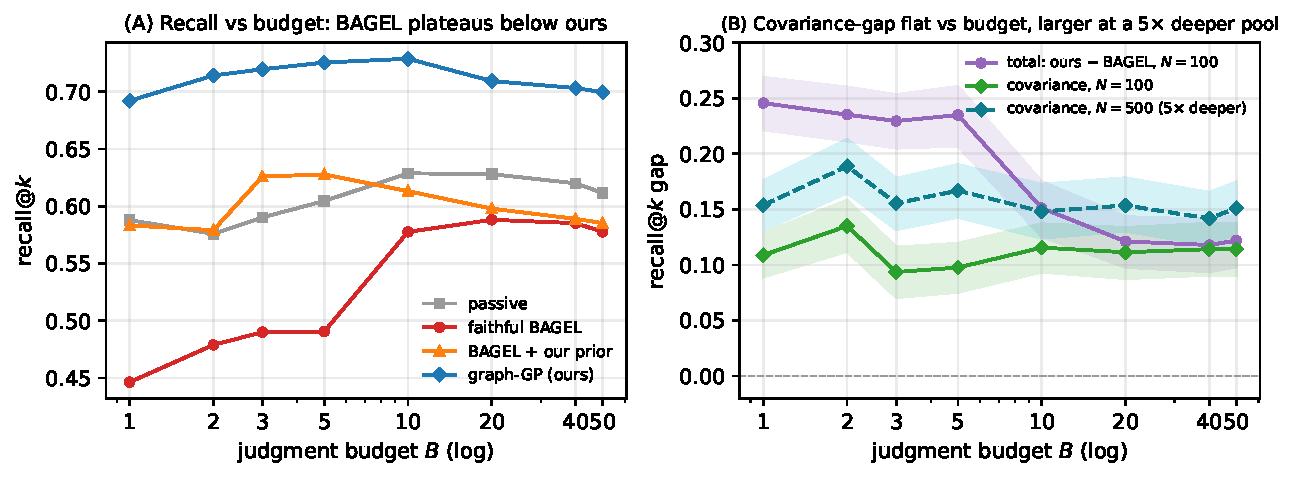
\includegraphics[width=.9\linewidth]{fig_bagel.pdf}
\caption{Faithful BAGEL vs.\ ours at matched judgment budget. \textbf{(A)} BAGEL plateaus about $0.12$ recall below
ours even at its native budget. \textbf{(B)} The total gap (ours$-$BAGEL) shrinks as BAGEL's zero-mean starvation
eases, but the covariance gap (same calibrated mean) is budget-invariant---$\approx+0.11$ at $N=100$ and, at a
$5\times$ deeper $N=500$ pool, flat and \emph{larger} at $\approx+0.15$. Bands are $95\%$ CIs.}
\label{fig:bagel}
\end{figure}
\begin{figure}[t]\centering
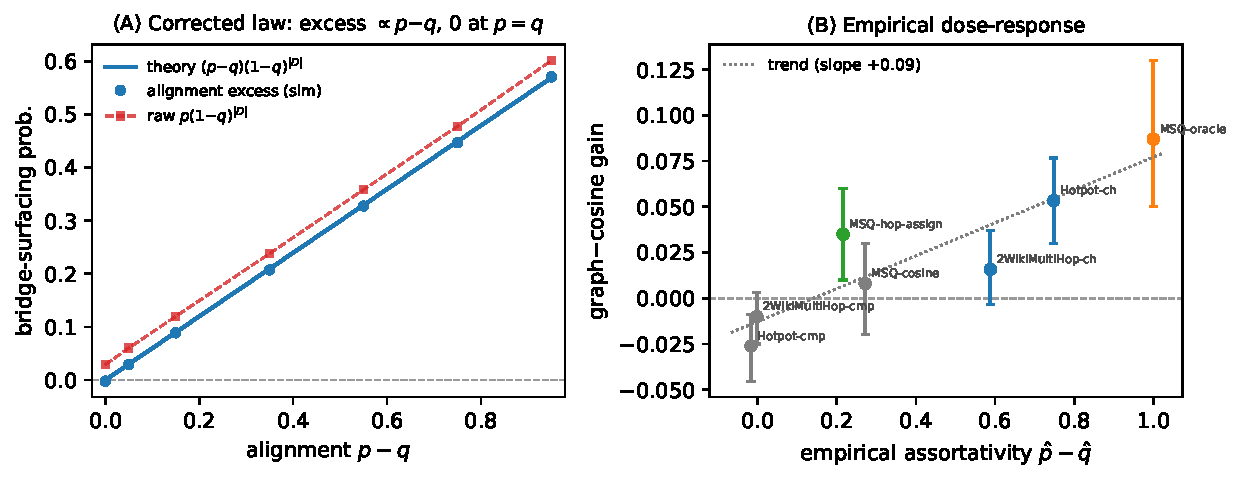
\includegraphics[width=.9\linewidth]{fig_alignment.pdf}
\caption{The alignment law in theory and data. \textbf{(A)} The alignment excess $(p-q)(1-q)^{|D|}$ vanishes at
$p=q$ and is linear in $p-q$, while the raw surfacing probability stays positive (chance surfacing).
\textbf{(B)} Real graph$-$cosine recall gain vs.\ empirical assortativity $\hat p-\hat q$, across datasets and graph
constructions: comparison questions ($\approx0$ assortativity, $\approx0$ gain), chained (positive), adversarial
MuSiQue cheap graphs (null) up to the oracle clique (maximal). Bars are $95\%$ CIs.}
\label{fig:align}
\end{figure}

\section{Both boundaries of the law}\label{sec:boundaries}
The theorem predicts \emph{where the graph should stop helping}, and the data oblige on both sides.

\paragraph{The neutral boundary: comparison questions.} Not every multi-hop question has a bridge. ``Comparison''
questions (``Who is older, X or Y?'') need two \emph{independently findable} facts and no linking passage. Here the
prior is already strong (passive recall $\sim0.8$) and there is no buried bridge to propagate to. The theorem then
predicts $\widehat A\approx0$ and no gain, and indeed the graph is neutral-to-slightly-negative on comparison
questions while helping chained ones by $+0.058\,[.040,.076]$ at $B=1$. Judging a mixed stream of $300$ chained
$+$ $300$ comparison questions traces the predicted boundary.

\paragraph{The adversarial boundary: MuSiQue, and a partial rescue.} MuSiQue is built to defeat structure: its
distractors are deliberately surface-similar to the golds, so cheap graphs (shared title, entity overlap,
cosine-decomposition) have $\hat p\approx\hat q$ and are null (graph$-$cosine $+0.008\,[\text{-}.02,.03]$ at three
hops). An oracle gold-clique graph recovers $+0.087\,[.05,.13]$---the two ends of the theorem's axis in one dataset.
Following the theorem's prescription (\emph{raise $p-q$}), we build the graph from the judge's \emph{own} reasoning:
decompose the question into sub-questions and ask the judge which sub-question each passage answers, then connect
passages that answer \emph{different} hops. This recovers a significant $+0.035\,[.01,.06]$ at three hops---about
$4\times$ the cosine graph and $40\%$ of the oracle headroom---where every surface graph is null. This spends extra
LLM calls to \emph{build} the graph, outside the judgment budget, so we report it as a proof of concept that
inferring structure from the judge's reasoning is the route to adversarial corpora, not as a budget-fair
competitor. The budget-fair version---elicit each passage's hop role \emph{in the same call} as its relevance
grade---is the natural sequel.

\section{An honest negative: why not adapt per query?}\label{sec:negative}
The obvious improvement is a gold-free gate that decides, \emph{per query}, whether to use the graph---switching it
on for bridge-questions and off for comparison-questions. It does not work, and the reason is worth stating
carefully because it is a statistical statement, not an engineering failure.

The per-query graph advantage is a \emph{small mean effect swamped by variance}: its query-level signal-to-noise
ratio is only $\approx0.1$--$0.2$. Consequently it is nearly unpredictable from gold-free features \emph{even under
an oracle that can see the labels when fitting the predictor}: a ridge regression of the per-query advantage on
alignment/reachability features achieves $R^2\approx0.03$--$0.05$. Two mechanistic hypotheses for a gate both fail:
the graph does \emph{not} amplify judge errors (the per-query advantage \emph{correlates $-0.17$} with anchor
reliability, the wrong sign for an error-amplification story), and confidence-gating the propagation to only
high-confidence labels \emph{hurts} by $0.030$ (the ``related,'' grade-$1$ labels carry useful propagation signal).
On the mixed stream the learned gate only \emph{ties} an always-on-graph policy ($+0.003$, not significant), while
the per-query \emph{oracle} gate has a real $+0.027$ of headroom that is simply not reachable from gold-free
features. The conclusion is a clean dichotomy: the structural gain is a \emph{distributional} property---a reliable
average over the deep-multi-hop regime, which is exactly what the alignment law describes---and \emph{not} a
per-query-predictable signal. The correct policy is therefore the simple one: use the graph throughout the
multi-hop regime it targets, and do not attempt per-query adaptivity, which is neither feasible nor needed.

\begin{stats}
This is a variance-components argument. Decompose the graph advantage into a between-regime mean (chained vs.\
comparison) plus a within-regime, query-level residual. The mean is real and estimable (that is the alignment law);
the residual has an $R^2$ near zero against any gold-free covariate, so no gate can exploit it. Reporting the
regime-level effect and \emph{declining} to claim a per-query one is the honest read of a low-$R^2$ residual---the
same discipline one would apply before claiming an interaction that the data cannot support.
\end{stats}

\part*{Part VI. Closing}
\addcontentsline{toc}{section}{Part VI. Closing}

\section{Discussion, and what a statistician should take away}\label{sec:disc}
The numbers are modest by design; the contribution is an \emph{account}. Four pieces fit together. (1)~A
mean/dependence decomposition: cheap semantics belong in the GP mean, corpus structure in the covariance, and
conflating them---using the graph to rank---is the mistake the field keeps making. (2)~A methodological detail with
real teeth: the graph covariance must be used in correlation form, or a variance-based sampler ignores exactly the
nodes that propagate. (3)~A proved alignment law that unifies, on a single axis $p-q$ estimated by assortativity,
the oracle ceiling and the adversarial failure, and predicts the neutral boundary. (4)~An honest map of where the
method helps (deep multi-hop with a chain-assortative graph), is neutral (independent-evidence questions), and is
only partially recoverable (adversarial corpora, via inferred structure), together with a variance-components reason
that per-query adaptivity is not on the table.

The deepest open direction is \emph{adaptive structure learning}: inferring the reasoning-chain graph from the first
few judgments---raising $p-q$ inside the budget rather than assuming a good graph is handed to us. The MuSiQue
hop-assignment result is a first instance. To a statistician the natural framing is a joint model in which each
judgment returns both a relevance grade and a role, the roles update a posterior over the block structure, and the
acquisition rule trades off learning the field against learning the graph that governs its covariance. That is the
sequel, and it is squarely a problem in Bayesian experimental design on an unknown dependence structure.

\subsection*{A one-page glossary}
\noindent\begin{tabular}{@{}p{0.28\linewidth}p{0.66\linewidth}@{}}
\toprule
Term & Meaning in this paper \\ \midrule
Passage & A short text chunk (one paragraph) that can be retrieved. \\
Gold passage & A passage that truly supports the answer (ground truth). \\
Bridge & A gold passage supplying a linking fact, textually dissimilar to the question. \\
Embedding $v_i$ & A unit vector for passage $i$; cosine $v_i^\top v_j$ measures topical similarity. \\
Judge / judgment & An expensive LLM call grading a passage's relevance $0/\tfrac12/1$. \\
Budget $B$ & Number of judgments allowed per query. \\
Prior mean $m_i$ & Calibrated cosine-to-relevance score; the GP mean. \\
Graph kernel $K^G$ & $(I+\lambda\mathcal L)^{-1}$, a GMRF/CAR covariance on the corpus graph. \\
Correlation form & $K^G$ rescaled to unit diagonal (\S\ref{sec:corr}). \\
UCB & $\arg\max_i\mu_i+\beta\,\mathrm{sd}_i$; the acquisition rule. \\
Alignment $p-q$ & SBM within-chain minus off-chain edge probability; estimated by assortativity. \\
recall@$k$ / completion & Fraction of gold in top $k$ / all gold in top $k$. \\
\bottomrule
\end{tabular}

\bibliographystyle{plainnat}
\bibliography{paperA}

\end{document}
